\section{Discussion}

% ideas I have
% opportunities for design/evaluation on crowdsourcing platforms and the need for this information to be widely shared
% parallels rai crowd workers are displaying compared to what's found in the literature --> the question of whether it's ethical to keep crowdsourcing in the future

\subsection{Design Implications}
% here we talk about specific design implications from the findings
\subsubsection{Front-load Worker Preparation Upon Platform Sign-up}
Our findings suggest that platforms should reconsider the minimal role they currently play in preparing workers for sensitive content tasks. While sign-up surveys and opt-in checkboxes are often treated as legal cover, workers emphasized that platforms have an ongoing responsibility to enforce protections and support well-being. One design implication is that platforms should offer structured opportunities for workers to express preferences and revisit them over time, rather than a one-time disclosure at sign-up. In addition, platforms could provide lightweight training or onboarding modules that introduce workers to common categories of sensitive content and prompt reflection about personal boundaries. Such training could serve both to help workers develop self-awareness and to improve data quality by reducing the likelihood of unanticipated harm mid-task. This implication resonates with prior work calling for platforms and companies to provide preparation and resources for content moderators~\cite{qian2025aura, steiger_psychological_2021, steiger2022effects}. 


\subsubsection{Increase Specificity to Ensure Sustainable Worker Responses}
We found that workers, task designers, and platforms all held incomplete or mismatched understandings of how warnings shape participation. Designers feared that warnings would deter participation, while workers consistently emphasized the value of specific details in making informed decisions. Our findings point to a design implication that risk disclosures should increase in specificity rather than remain generic. Specificity may strengthen sustainability by protecting workers from unexpected harms and by reinforcing the reputational standing of task designers, since prior work has shown that reputation is a critical factor in sustaining participation and trust in crowdsourcing~\cite{gaikwad2016boomerang, irani2013turkopticon}. Future work could explore tools that assist task designers in creating richer disclosures, such as AI-driven keyword generation, taxonomies of severity, or prompts informed by prior worker feedback. By reframing specificity as a contributor to both worker well-being and long-term platform sustainability, designers can move away from the assumption that detail undermines participation. 

\subsubsection{Encourage Feedback Through Facilitating Worker-Task Designer Relationship-Building}
Feedback emerged as one of the few areas of relative agreement among all stakeholders. Workers valued it as a rare moment of agency, task designers viewed it as essential for improving warnings, and platforms saw it as a way to maintain trust. Yet feedback is currently under-supported in most platform designs. We suggest that platforms experiment with mechanisms that actively encourage feedback and deepen worker–task designer relationships, for example, by integrating feedback prompts into the workflow, offering compensation for reflective responses, or highlighting when feedback leads to concrete changes. These mechanisms should be designed with sensitivity to workers’ well-being, allowing them to decline feedback after distressing tasks without penalty. Prior work has examined the importance of task-designer–worker relationships in shaping trust and quality in crowdsourcing~\cite{irani2013turkopticon, qian2025locating}, but the role of feedback in mitigating risk disclosure failures remains underexplored. Our findings suggest this as a promising area for both empirical evaluation and design innovation. Notably, we already observe early platform changes in this direction (see Figure \ref{fig:prolific-feedback} of Prolific's new feature for increased feedback from workers), but systematic evaluation could better inform practice. 
\begin{figure}[htbp]
    \centering
    % Left image
    \begin{minipage}{0.48\textwidth}
        \centering
        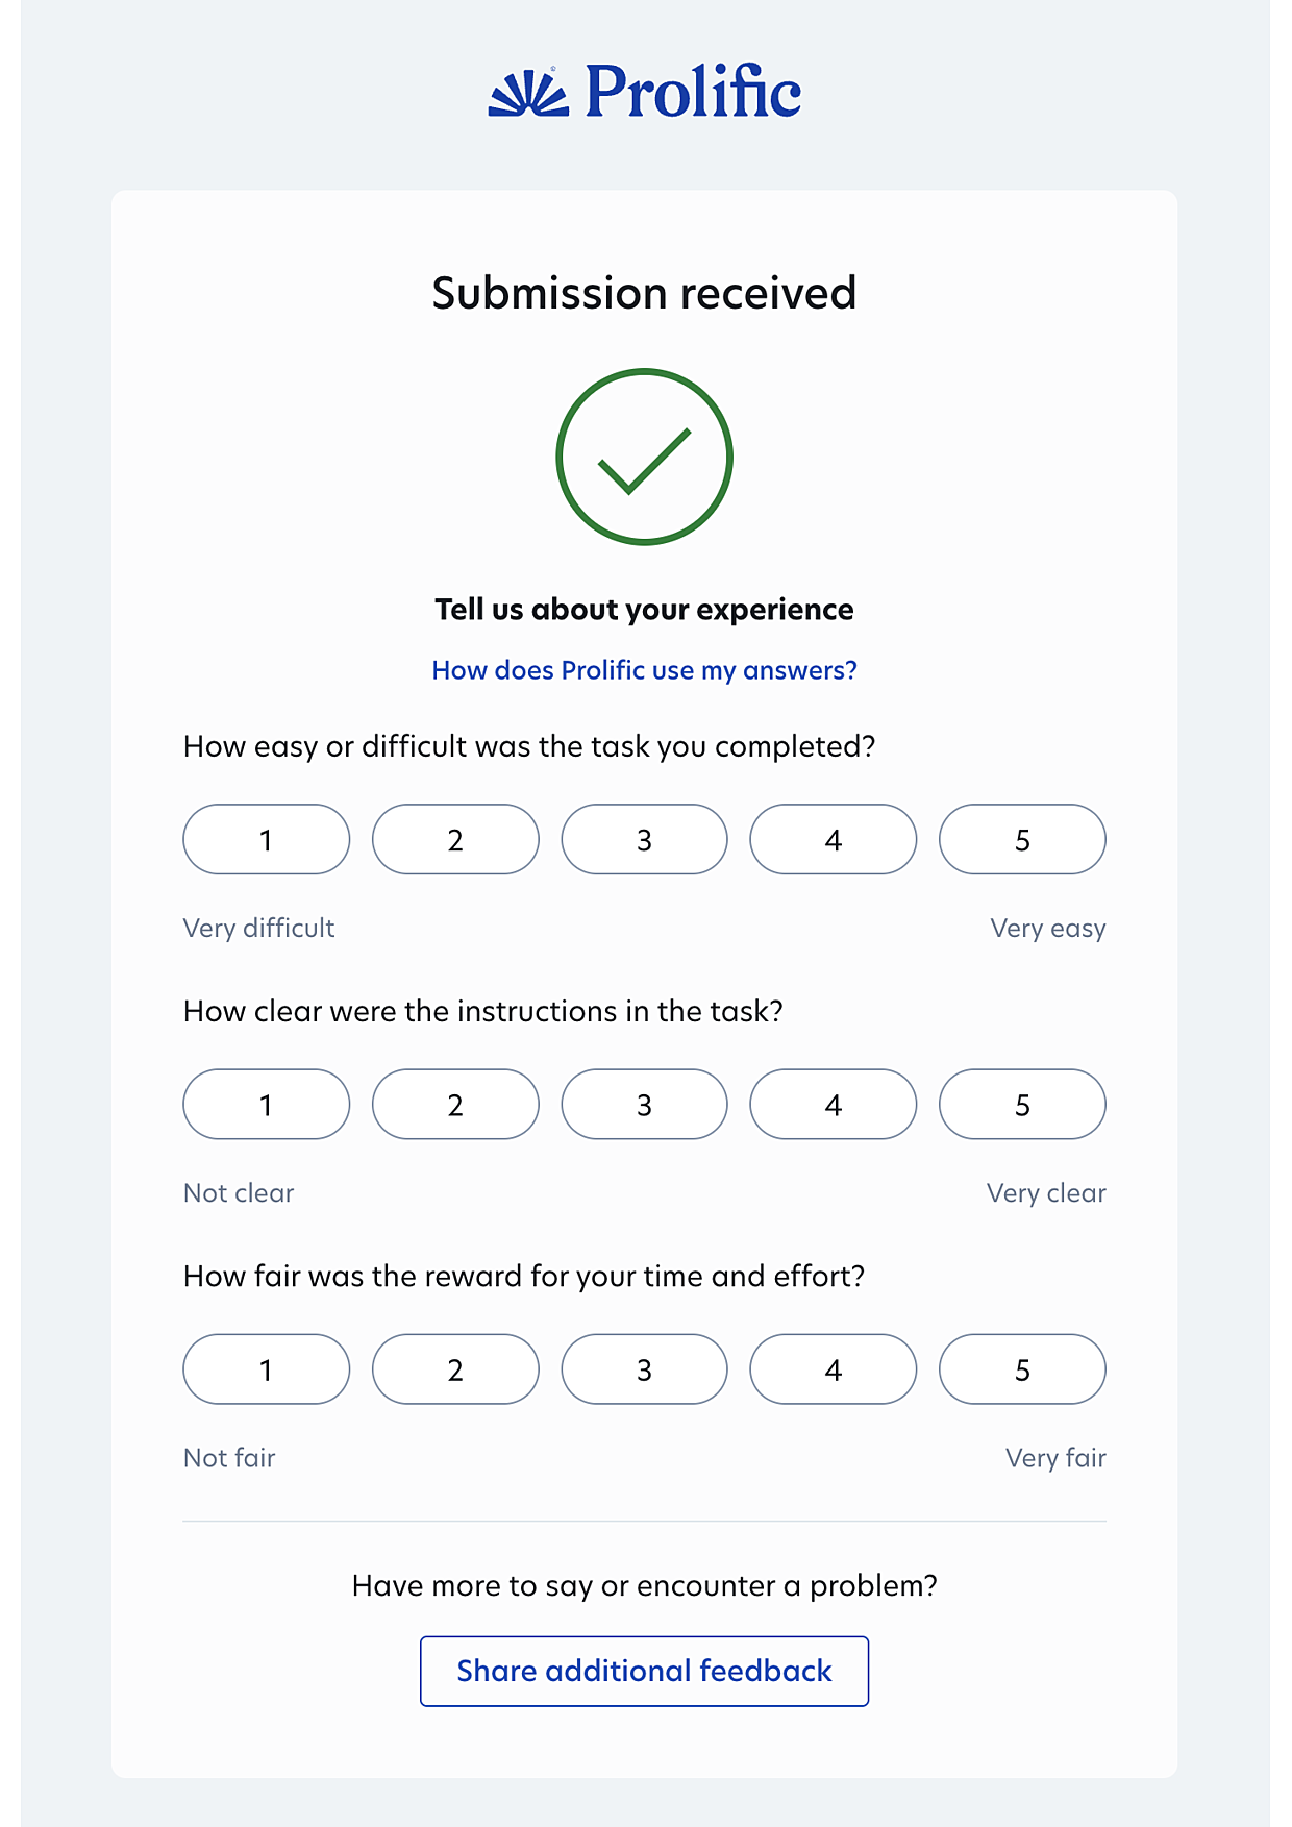
\includegraphics[width=\textwidth]{figures/prolific_feedback.pdf}
        \caption{Option to provide feedback on Prolific \protect\footnotemark}
        \label{fig:left}
    \end{minipage}
    \hfill
    % Right image
    \begin{minipage}{0.48\textwidth}
        \centering
        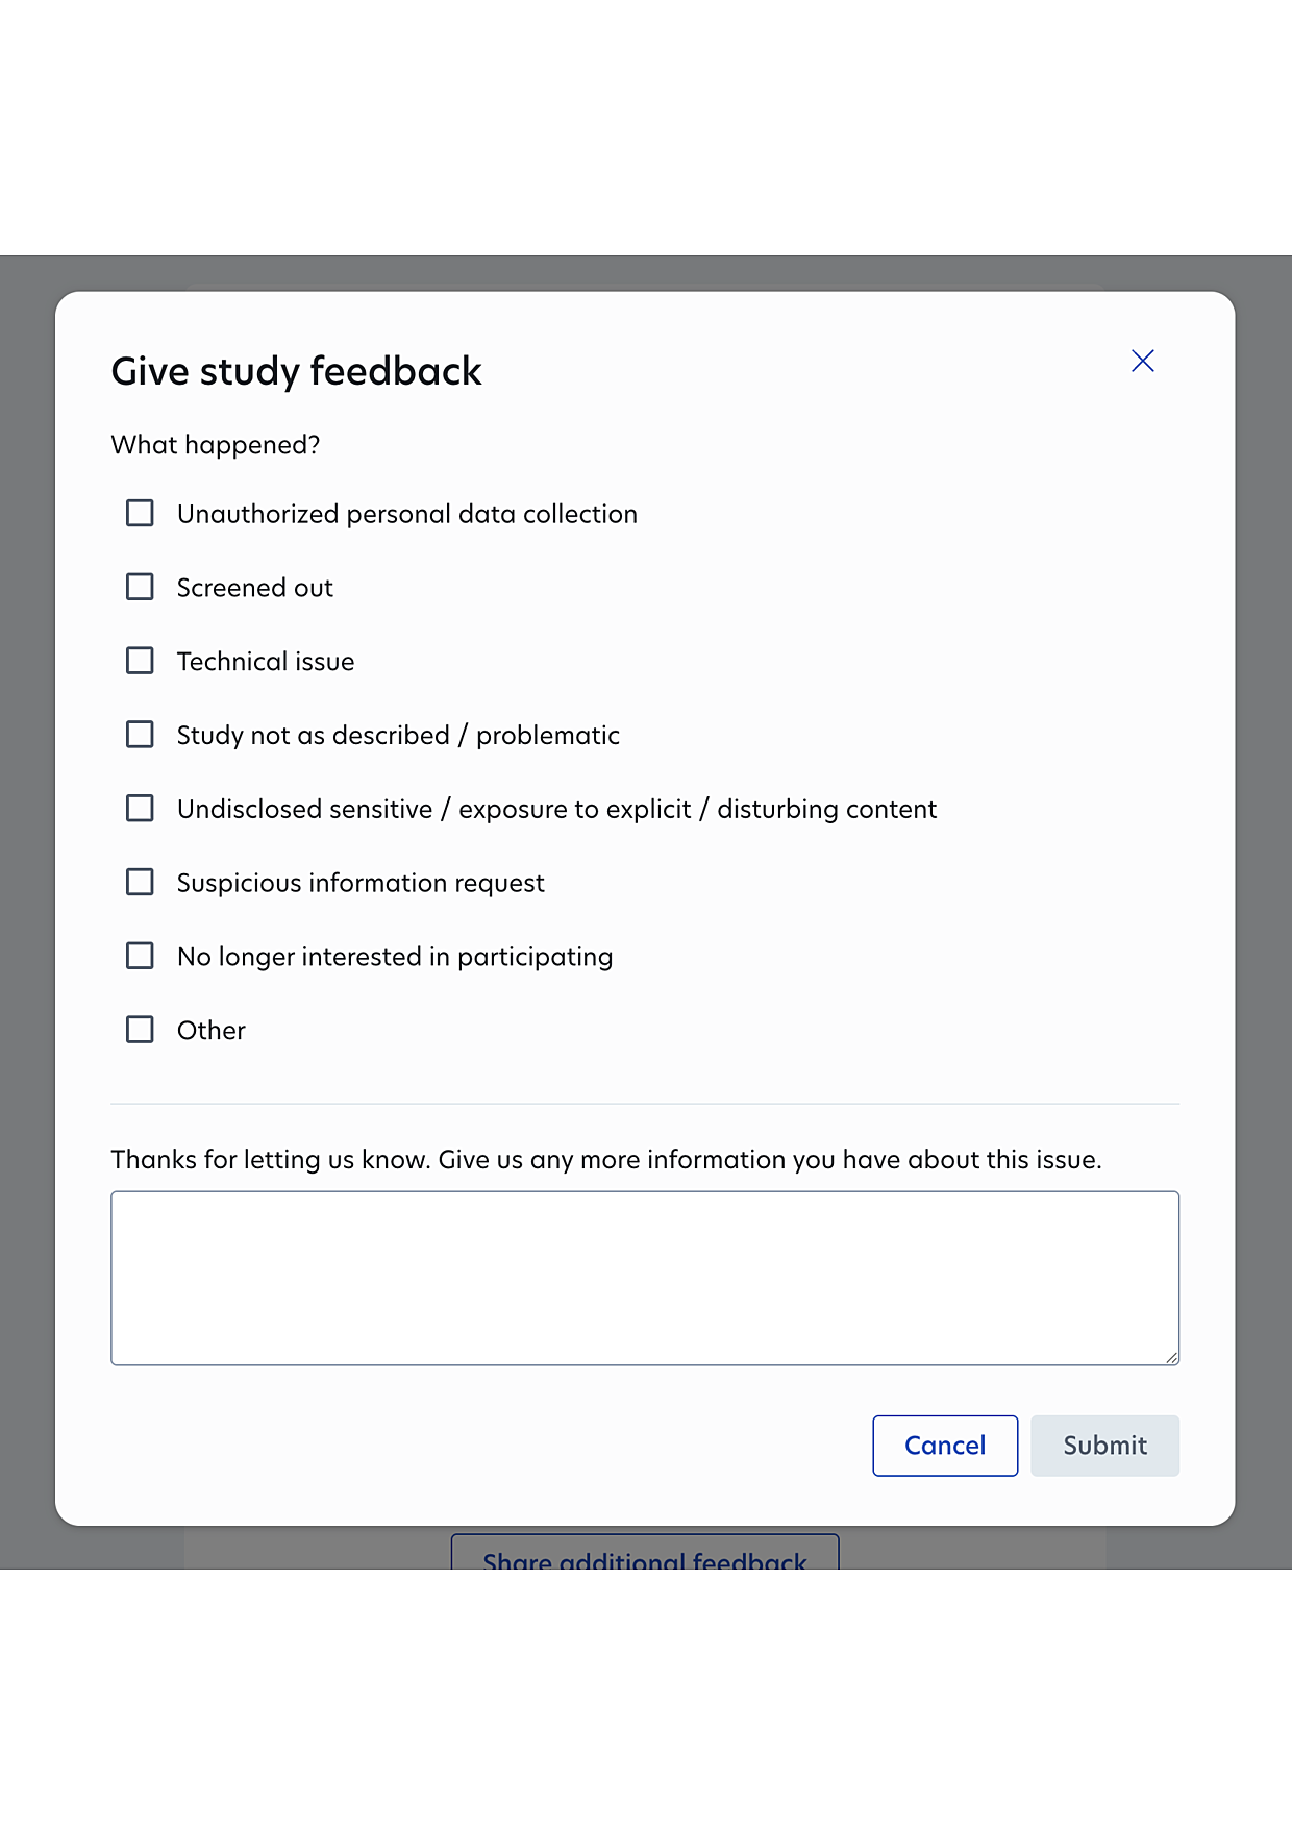
\includegraphics[width=\textwidth]{figures/prolific_feedback_extra.pdf}
        \caption{Option to provide extra feedback on Prolific}
        \label{fig:right}
    \end{minipage}
    \caption{Most recent changes to how Prolific collects feedback from workers on tasks}
    \label{fig:prolific-feedback}
\end{figure}

\footnotetext{Documented by an author completing a task on September, 2025}
\subsection{Negotiated Responsibility in Risk Disclosure}
% discussion of risk disclosure being a site of negotiated responsibility between our 3 groups. Our findings show how these actors hold different assumptions about who is responsible for identifying and mitigating harm. Acknowledging this dynamic allows us to shift our design question from how risk should be disclosed to who decides, when, and on what basis? 
Our study reveals that risk disclosure in AI data work is a socially negotiated process among workers, requesters, and platforms. We confirm previous work that found these groups hold distinct and at times conflicting assumptions about who should identify, assess, and communicate risks \cite{fieseler_unfairness_2019}. Workers often assume that task requesters or platforms have already vetted tasks for harm, while task designers may assume that workers bear responsibility for self-selecting out of sensitive content. Platforms, meanwhile, frequently promote a vision of shared responsibility while retaining control over infrastructure and moderation policies. These mismatches lead to practical gaps in risk disclosure and reinforce structural ambiguities around accountability \cite{Suchman2002LocatedAccountabilities, widder_dislocated_2023}.


This ambiguity invites us to reframe the design challenge. Rather than simply asking how risk should be disclosed, we must interrogate who decides, when, and on what basis. These questions draw attention to power asymmetries embedded in crowdsourcing platforms. Workers have limited opportunities to contest or shape disclosure practices, even as they bear the brunt of poorly disclosed risks. Task designers may want to warn workers, but are constrained by platform guidelines or unsure of what they are permitted to disclose. Platforms can offer guidelines or tools, but are often opaque about how risks are evaluated or escalated internally~\cite{roberts2019behind}.

By conceptualizing risk disclosure as a site of negotiated responsibility, we can open new design directions. Future tools might aim not just to standardize disclosure formats, but to mediate disagreement and dialogue across stakeholder boundaries \cite{fieseler_unfairness_2019}. For example, platforms could surface discrepancies in risk perception between task creators and workers, or allow workers to annotate disclosures with feedback. Designing for this kind of deliberation requires acknowledging that disclosure is a form of boundary crossing~\cite{Suchman2002LocatedAccountabilities}, not simply a transfer of information, but a process shaped by contested expertise, values, and institutional constraints.

Moreover, understanding these negotiations requires us to move beyond individualistic framings of responsibility. Instead, we can draw on theories of distributed or relational accountability, which emphasize how ethical obligations are produced through collective, situated practice~\cite{marwick2014networked}. Such a lens complicates the assumption that risks can be fully known or managed in advance, and suggests the need for systems that are reflexive and adaptive over time.


\subsection{Supporting Worker Well-Being Beyond Risk Disclosure}
% where we can talk about workers needing more support (helpline isn't enough) and also what are platform gonna do if they provide a number of a product manager you can call? unrealistic?
While task-level risk disclosures are a critical starting point, they are only one component in a broader ecology of worker well-being. Our findings reveal that workers, even when appreciative of disclosure efforts, continue to face harm that is structural, cumulative, and poorly addressed by current platform support. Many participants described psychological strain from sustained exposure to distressing content, difficulty disengaging from harmful tasks, and a lack of avenues for recovery. Helplines and automated filters offer some relief, but fall short of meeting the scale and complexity of workers’ needs~\cite{qian2025aura, spence2023content, steiger2022effects}.

In particular, workers expressed a desire for more robust pre-task support. This includes not only clearer disclosures but also access to training and reflection tools that could help them assess personal thresholds for harm and prepare emotionally for the work. Existing research on content moderation and trauma-informed design points to promising strategies here, such as onboarding experiences~\cite{steiger_psychological_2021, steiger2022effects}, exposure reduction ~\cite{dang_but_2018, das_fast_2020, Iyadurai2018PreventingIntrusiveMemories, holmes_can_2009}, and the reconsideration of broader career pathways for workers~\cite{qian2025aura} that could be adapted for the crowdsourcing context.

Post-task care is an even more underexplored frontier. Some workers suggested mechanisms such as debriefing spaces, access to mental health resources, or the ability to pause or escalate after encountering disturbing content. However, the logistics of such support remain unclear: who would provide it, under what funding model, and with what safeguards? In an industry defined by just-in-time labor and minimal worker protections, offering meaningful well-being resources challenges the very business models that platforms depend on~\cite{gray2019ghost}.

Moreover, the workers most vulnerable to psychological harm are often those with the least power to request accommodations. Crowdworkers span geographies, languages, and socioeconomic contexts—factors that mediate not only their exposure to harm but also their ability to access care. Designing for worker well-being thus requires a deeply intersectional approach, one that foregrounds structural inequalities rather than treating harm as a purely individual experience~\cite{miceli2022data}.

\subsection{Limitations of Co-Designing for Risk Disclosure in RAI Content Work}
% of whether we should crowdsource RAI content work}
% cite implication to not design paper
% what type of task should be crowdsourced
% should be crowdsource at all
% can directly call out our limitation as a co-design study here, with power imbalance of workers
% from Hong this report has definitions of platform: https://www.ilo.org/sites/default/files/wcmsp5/groups/public/%40dgreports/%40dcomm/%40publ/documents/publication/wcms_645337.pdf
% - we focus on the complexities of this design space, but there is an itneresting question about whether it's effective or ethical to crowdsource this work
% - maybe we can crowdsource, but we don't make this into microtasks
% - in terms of what is effective, this does align with what our task designers want and some of our findings showed that some workers are open to this too
% - of course this will take away power from platforms
% - in terms of the ethics (cite literature) 
% this is sort of a policy implications section

Our findings also surface a deeper question: \textbf{Should we crowdsource risky or sensitive AI content work in the first place?} While our study focuses on improving the design of risk disclosures, it cannot sidestep broader concerns about whether the task environment itself is appropriate or just. As prior literature has shown, microtasking can fragment judgment, mask ethical complexity, and devalue the expertise required to make nuanced content decisions~\cite{berg2018digital}. These concerns are amplified in the context of RAI development, where annotation decisions can shape downstream system behavior~\cite{wang2022whose, diaz2022crowdworksheets}.

Several task designers in our study justified crowdsourcing on the basis of diversity and scalability, noting that crowdworkers provide valuable perspectives and can be engaged more flexibly than full-time staff. Some workers echoed this, citing financial need or interest in meaningful participation. Yet the same workers also described feeling isolated, underpaid, and unsupported when engaging with emotionally fraught tasks. This suggests that current practices may extract value from worker insight without adequately compensating for the associated risks. Rather than rejecting crowdsourcing altogether, one alternative is to rethink how it is done. For example, longer-form or collaborative annotation formats might give workers greater context and control. Task structures could emphasize care and deliberation over speed, perhaps shifting away from performance-based incentives and toward reflective judgment. Some of these ideas mirror trends in community moderation or participatory research, where contributors are treated as co-creators rather than disposable labor~\cite{wang2022whose}.

However, such changes would likely challenge platform logics and economic incentives. Implementing slower, more dialogic forms of labor requires reconfiguring not only interface design, but also compensation structures, labor policy, and institutional accountability. These are not merely technical or logistical challenges, but ethical ones. We therefore join prior scholars in calling for greater scrutiny of whether certain types of work should be crowdsourced at all—and under what conditions it can be considered just, humane, and sustainable~\todo{not sure what citation to add here}. 
